\section{Gruppi di lavoro agili}
Prima di addentrarci nella spiegazione del perchè sono nati i gruppi di lavoro agili facciamo un riassunto di quello che è il pensiero elaborato fino ad ora:
\begin{itemize}
    \item Sviluppare software in gruppo è difficile (The Tar Pit): poichè le attività sono difficilmente separabili la complessità del coordinamento aumenta col quadrato del numero di componenti (Legge di Brooks)
    \item La soluzione gerarchica: la squadra di lavoro gioca per il progettista (cattedrale/sala operatoria)
    \item L'esistenza di progetti open source con migliaia di partecipanti sembra mettere in dubbio la Legge di Brooks
    \item L'organizzazione di questi gruppi è molto decentrata e le idee progettuali vengono da più parti (bazaar)
    \item Legge di Linus: le attività di verifica e convalida sono parallelizzabili
    \item In realtà però la Tar Pit e il caso sono sempre in agguato: più che dei bazaar disordinati, i progetti distribuiti tendono più ad assomigliare a dei kibbutz, con valori tecnologici condivisi e regole di partecipazione e sviluppo forzate da strumenti software
\end{itemize}

Negli anni '90 (dove UML era padrone) nascono molti approcci legati soprattutto dal fastidio per l'eccessiva enfasi data alla documentazione del processo di sviluppo.
Nascono così:
\begin{itemize}
    \item eXtreme Programming (XP)
    \item Scrum
    \item DSDM
    \item Adaptive Software Development
    \item ...
\end{itemize}
I ricercatori dell'ingegneria del software hanno sempre messo in evidenza la crucialità del processo di sviluppo e studiato cicli di vita iterativi.\\
Il manifesto della \textbf{Programmazione Agile} viene pubblicato nel 2001, ed esprime i seguenti concetti:
\begin{enumerate}
\item Individui e interazioni \textgreater\space Processi e strumenti
\item Software funzionante \textgreater\space Documentazione esaustiva
\item Collaborazione cliente \textgreater\space Negoziazione contratti
\item Rispondere al cambiamento \textgreater\space Seguire un piano
\end{enumerate}
Tutti questi punti sono però \textbf{molto generici e idealistici}, e sono sì belli, ma poco applicabili. Il più concreto di questi è forse il punto 4, perchè riconosce il fatto che è molto facile sbagliare la pianificazione. È meglio quindi salvare risorse per potersi adattare a nuove situazioni.\\
\noindent Al contrario di quanto si è portati a pensare, agile non significa il rifiuto dei processi, ma piuttosto il rifiuto di continue verifiche e benchmark come misura della qualità di quanto prodotto. Quello che fanno gli agilisti è sostituire al canone fatto di processi e misurazioni un canone con dei principi astratti più o meno condivisibili. \\
Tra i più importanti principi agili troviamo:
\begin{itemize}
    \item Rilasciare software di valore, fin da subito e in maniera continua (non c'è quindi solo una consegna finale)
    \item Consegniamo frequentemente software funzionante
    \item Il software funzionante è la principale misura di progresso 
    \item Cambiamenti nei requisiti anche negli stadi avanzati
    \item Committenti e sviluppatori devono lavorare insieme quotidianamente
    \item Conversazione faccia a faccia
    \item Individui motivati e ben supportati
    \item Sviluppo sostenibile: essere in grado di mantenere indefinitamente un ritmo costante
    \item Eccellenza tecnica
    \item Team che si auto-organizzano
    \item A intervalli regolari il team riflette su come diventare più efficace
    \item La semplicità - l'arte di massimizzare la quantità di lavoro non svolto - è essenziale
\end{itemize}
Il manifesto non è un metodo, nè veramente un 'programma': parla ai cuori più che alle teste degli sviluppatori. È la dichiarazione di un disagio (non voglio essere pagato per scrivere documenti che nessuno legge) e la prefigurazione di
un’utopia (il paradiso dei programmatori). I metodi agili (principalmente XP e Scrum) fanno invece proposte concrete (non sempre facilmente identificabili come in linea col manifesto. . . )

\subsection{Principi agile nella pratica}
Questi principi nell'implementazione in canoni agile si traducono nelle seguenti prescrizioni:
\begin{itemize}
\item Team \textbf{piccoli} e \textbf{auto-organizzati}, senza manager tradizionali, ma facilitatori (evitano che l'auto-organizzazione diventi anarchia)
\item Rifiuto di azioni e decisioni \textbf{big upfront}, sviluppo interattivo aperto alla variazioni in corso d'opera: cerco di non prendere decisioni troppo importati a meno che non posso fare altrimenti. Mi preoccupo di possibili cambiamenti solo quando il problema si pone effettivamente. Spesso no big upfront è noto con YAGNI (you aren't gonna need it), quindi non sviluppo una cosa finchè non è completamente chiaro che ne ho bisogno. Cerco quindi di evitare l'\textbf{over engeneering}
\item Misura e controllo del processo di sviluppo, con pianificazioni con orizzonti temporali e funzionali ridotti: ovvero mi concentro molto su quello che farò oggi, non mi preoccupo di quello che farò fra 2 settimane
\item Enfasi su testing, intesa come tecnica di sviluppo.
\end{itemize}
La parte più problematica è la partecipazione della committenza, che infatti è interpretata in maniera molto diversa dai vari approcci agili.

\subsubsection{Enfasi sul testing}
I requisiti sono sostituiti dalle \textbf{User Stories}, ovvero dei template di frasi che il committente compila.
\begin{center}
\textit{As a} \texttt{USER TYPE} \textit{I want} \texttt{FUNCTIONALITY} \textit{so that} \texttt{MOTIVATION}
\end{center}
Queste frasi vengono usate per capire cosa bisogna fare e per valutare se vale davvero la pena farlo.\\
La specifica che l'ingegneria classica produce è invece sostituita da \textbf{casi di test}, che vengono associati alle user stories. Il mio scopo è quindi quello di far passare i test, ovvero sto facendo \textbf{Test Driven Development (TDD)}.\\
Deve quindi essere chiaro che il \textbf{test non è un elemento di verifica}.

\subsection{Scrum}
Scrum vuol dire mischia (tipo Rugby). Tutta la metodologia Scrum è descritta in un piccolo manuale di 17 pagine, molto schematico e sintetico.\\
Questo framework prescrive alcune regole:
\begin{itemize}
\item \textbf{Team piccoli}: 7+-2 persone. Il team è auto-organizzato, ma ci devono essere un \textbf{product owner} e uno \textbf{scrum master}.
\item \textbf{Presenza di un \textbf{product owner}}: è il membro del team che funge da rappresentate del committente (fa comunque anche gli interessi della propria azienda), in modo tale da non dover scomodare il committente vero e proprio. Funge anche da interfaccia con il committente. Gestisce il backlog. Ciò è necessario perchè Scrum prescrive la necessità di ripianificare spesso.
\item \textbf{Presenza di uno Scrum Master}: è il facilitatore del gruppo. Cerca di ovviare a problemi di sviluppo, ma anche logistici ecc. Ma esiste anche per fare rispettare i principi dello Scrum, in modo da far funzionare meglio lo Scrum stesso.
\item \textbf{Membri del team}: oltre che a programmare, devono fare anche le stime, che sono fondamentali.
\end{itemize}

\subsubsection{Pianificazione}
Non serve niente pianificare a lunghi periodi, perchè si rischia di sbagliare. È meglio pianificare a brevi intervalli, in modo tale da avere una pianificazione corretta e quindi Utile.\\
Nello sviluppo agile si creano delle \textbf{epopee} (insieme di user story) che si sviluppano in sprint con \textbf{lunghezza prefissata} di 1-3 settimane. Queste permette di avere una velocità costante e di pianificare quindi correttezza. So che comunque alla fine di questo sprint dovrò rilasciare qualcosa, anche se non del tutto conforme a quanto pianificato.\\
Durante lo sprint non è possibile rinegoziare o aggiungere features, al limite si ricomincia lo sprint. Si chiama \textbf{closed window rule}.\\
Per pianificare, scelgo una user story che è sicuramente chiara a tutti. A questa user story assegnerò un punteggio di 1. Esprimerò la complessità di tutte le altre user stories in relazione alla story di valore 1. Ogni membro del team fa una stima in segreto delle user story e la tiene segreta. Si scoprono le stime e poi si discute \textbf{insieme} sulla stima definitiva. Questa metodologia si chiama \textbf{planning poker}.\\
Le riunioni sono \textbf{timeboxed}, ovvero hanno una lunghezza prefissata. Quando si discute, sono presenti dei \textbf{pigs}, ovvero delle persone direttamente interessate che hanno voce in capitolo su una decisione, e dei \textbf{chicken}, ovvero persone che possono dare solamente un'opinione.

\subsubsection{Riunioni}
Sono prescritte le seguenti riunioni:
\begin{itemize}
\item \textbf{Daily stand up}: (15 min ogni giorno) Cosa abbiamo fatto ieri, cosa facciamo oggi, ci sono impedimenti?
\item \textbf{Planning}: (ogni 1-5 giorni). Pianificazione di uno sprint, definizione dello sprint backlog con stima per ogni epopea/storia
\item \textbf{Retrospettiva}: (circa 30 min) Alla fine di uno sprint, per migliorare i processi.
\item \textbf{Review}: (1 ora) Alla fine di uno sprint, presentazione del lavoro agli stakeholder (quindi anche al cliente).
\end{itemize}

\subsubsection{Tecniche di lavoro}
Si usano alcune tecniche di programmazione, provenienti sopratutto dall'eXtreme programming.\\
Molte di queste tecniche sono utilizzabili e hanno senso solamente se implementate tramite tools e \textbf{framework automatici}, come Git, Junit, ecc.
\paragraph{Pair Programming}
	È presente un \textbf{pilota} (colui che ha la tastiera) e un \textbf{copilota} (che dice cosa cosa fare e cosa scrivere). In questo modo, si è forzati a esplicitare cosa si vuole fare, e il codice scritto deve passare per almeno 2 persone. Ovviamente ci si da il cambio con un certo intervallo di tempo. Può sembrare una perdita di tempo e soldi, ma studi dimostrano che la produttiva è solo leggermente inferiore, a fronte di una qualità del codice più alta. In questo modo, poi, ci sono più persone che conoscono una certa codebase.
	
\paragraph{Codice Condiviso}
Tutto il codice deve essere accessibile e modificabile da ogni membro del team. Questo può essere estremante dannoso, ma i metodi agile pongono numerose protezioni per accorgersi di eventuali danni, come la \textbf{continuos integration} e il \textbf{TDD}.\\ La ragione dietro ciò è dare la priorità al software funzionante per avanzare nel progetto, piuttosto al dare a ogni persona la "colpa" per ogni singolo malfunzionamento.\\
Attenzione a non confondere la condivisione del codice come ragione per rinunciare all'\textbf{Information Hiding}.

\paragraph{Refactoring}
Riscrittura di un pezzo di codice senza cambiarne le funzionalità. Per essere sicuro di avere le stesse funzionalità, mi basta controllare che passi gli stessi test (vedi TDD). Molte delle operazioni di refactoring (come cambiare il nome una variabile) hanno dei metodi standard per essere implementati, anche in modo automatico (come per il cambio di nome).\\
Il refactoring ha l'obiettivo di generalizzare il codice scritto, anche mediante l'ausilio del catalogo dei \textbf{code smell}, ovvero delle bad practise di programmazione (come la duplicazione del codice) che andrebbero rimosse.

\paragraph{Test Driven Development (TDD)}
Non è assolutamente una tecnica di verifica, ma una tecnica di progettazione.\\
Funziona più o meno così:
\begin{enumerate}
\item Aggiungo un test
\item Ripeto tutti i test di assicurandomi che il test fallisca
\item Scrivo il codice per fare passar il test
\item Ripeto i test, che dovrebbero passare
\item \textbf{Refactoring}, mantenendo il funzionamento del test
\item Da capo
\end{enumerate}
Eventuali bug vanno esaminati e trasformati in caso di test.\\ Si svolgono test di unità tramite appositi framework, che metto a disposizione suite con mock ecc.

\paragraph{Velocity Tracking}
La velocità è una caratteristica del mio gruppo di lavoro, che riesco a conoscere con il tempo, facendo progetti. Il gruppo deve quindi costantemente monitorare il progresso, per vedere se in linea con quanto ci si aspetta.\\
Il meccanismo principale che mi permette di misurare il progresso è la \textbf{task board} come ad esempio il \textbf{kanban}. E la tipica board divisa in colonne (ex. Da Fare, In Lavorazione, Fatto). Si possono prevedere anche limiti di numerosità per colonna.\\
\begin{figure}[H]
	\centering
	 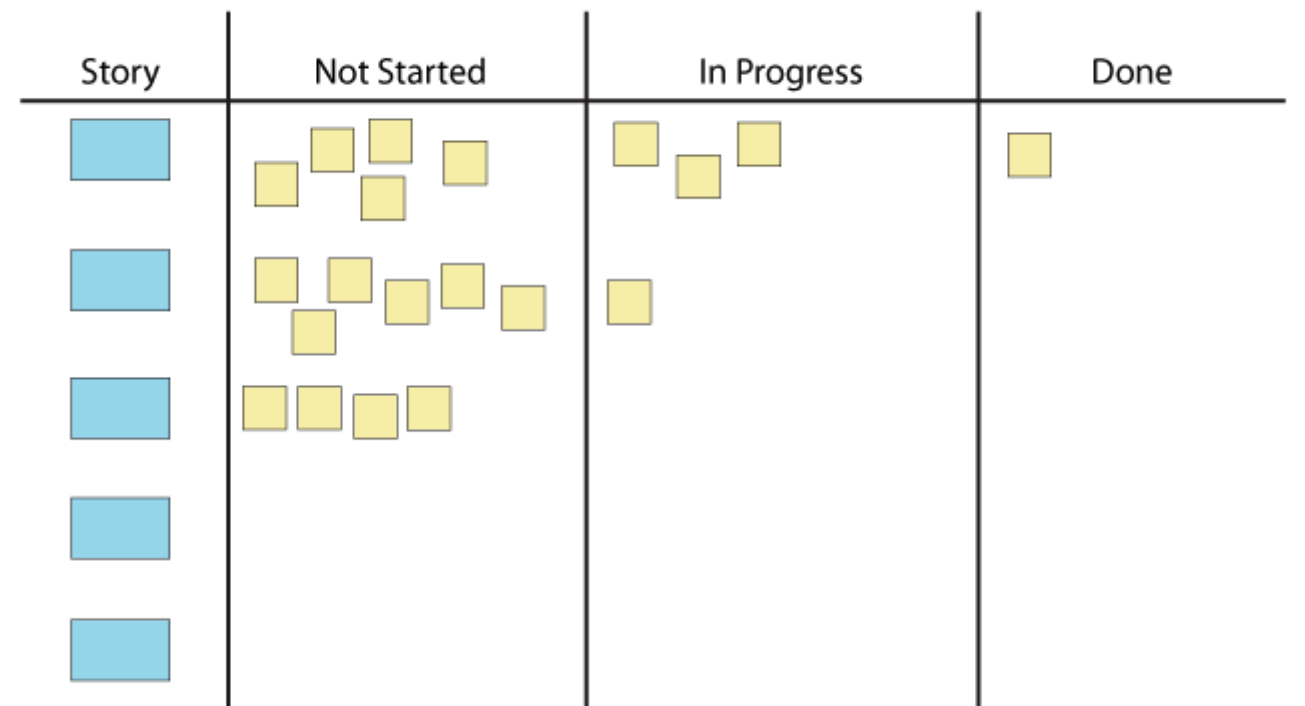
\includegraphics[width=\linewidth]{img/board.png}
	 \caption{Task board}
\end{figure}
L'idea è di tenera traccia di cosa si è fatto e di cosa manca fare. Tendenzialmente, nelle ascisse si tende a mettere una misura temporale, e si va a comporre il \textbf{burndown chart}.
\begin{figure}[H]
	\centering
	 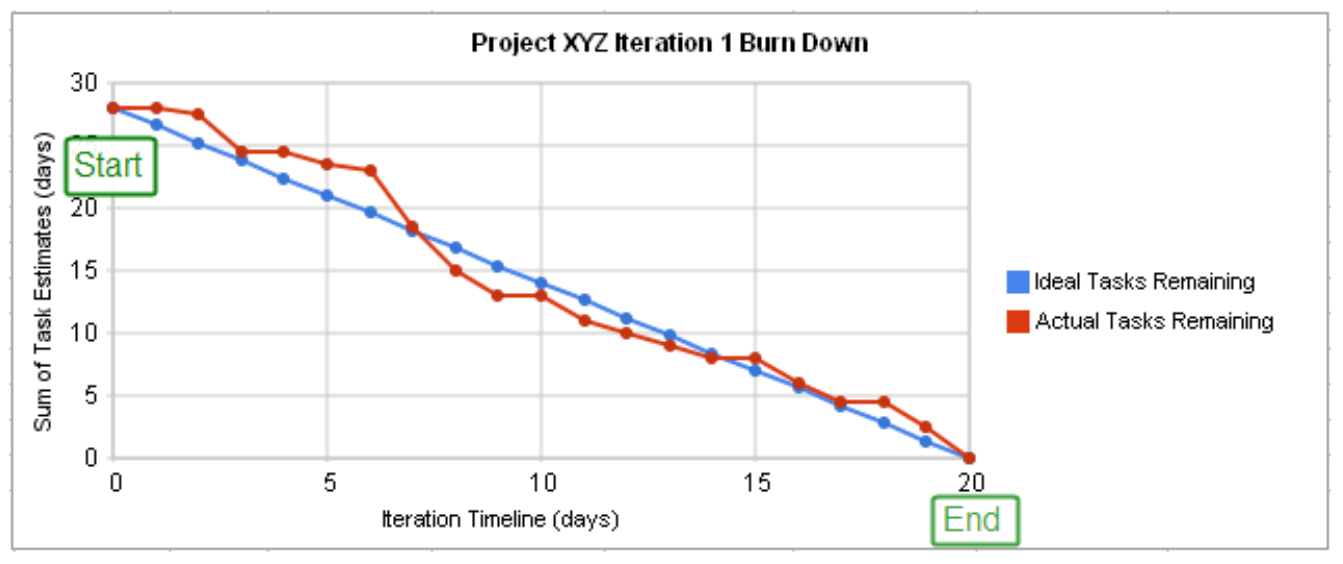
\includegraphics[width=\linewidth]{img/burnDown.png}
	 \caption{Burndown Chart}
\end{figure}
Quello che faccio solitamente è tenere traccia dello scostamento rispetto alla pianificazione lineare.\\
Una approssimazione per calcolare il tempo nelle ascisse è usare i giorni uomo, ad esempio per un sprint di 2 settimane con sei programmatori abbiamo \texttt{6 programmatori \textbf{x} 5 giorni a settimana \textbf{x} 2 settimane \textbf{/} 3}. Il diviso 3 serve perchè i meeting ecc portano via circa un terzo della giornata.
